% Created 2023-03-06 Mon 14:30
% Intended LaTeX compiler: pdflatex
\documentclass[11pt]{article}
\usepackage[utf8]{inputenc}
\usepackage[T1]{fontenc}
\usepackage{graphicx}
\usepackage{longtable}
\usepackage{wrapfig}
\usepackage{rotating}
\usepackage[normalem]{ulem}
\usepackage{amsmath}
\usepackage{amssymb}
\usepackage{capt-of}
\usepackage{hyperref}
\usepackage{eecstex}
\usepackage{float}
\usepackage[export]{adjustbox}
\author{Bryan Ngo}
\date{\textit{<2023-03-02 Thu>}}
\title{EE 105 Lab 03}
\hypersetup{
 pdfauthor={Bryan Ngo},
 pdftitle={EE 105 Lab 03},
 pdfkeywords={},
 pdfsubject={},
 pdfcreator={Emacs 28.2 (Org mode 9.6.1)}, 
 pdflang={English}}
\begin{document}

\maketitle
\tableofcontents


\section{DC Simulation Values}
\label{sec:orge2886f3}

\begin{figure}[H]
\centering
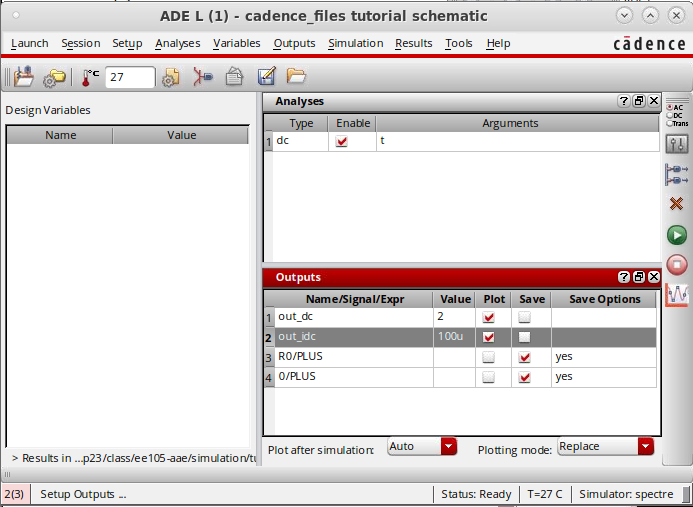
\includegraphics[width=0.7\textwidth]{./dc_sim.png}
\caption{\label{fig:dc_sim}DC simulation parameters.}
\end{figure}

\section{Formatted Plot for AC Magnitude Response}
\label{sec:org501c83f}

\begin{figure}[H]
\centering
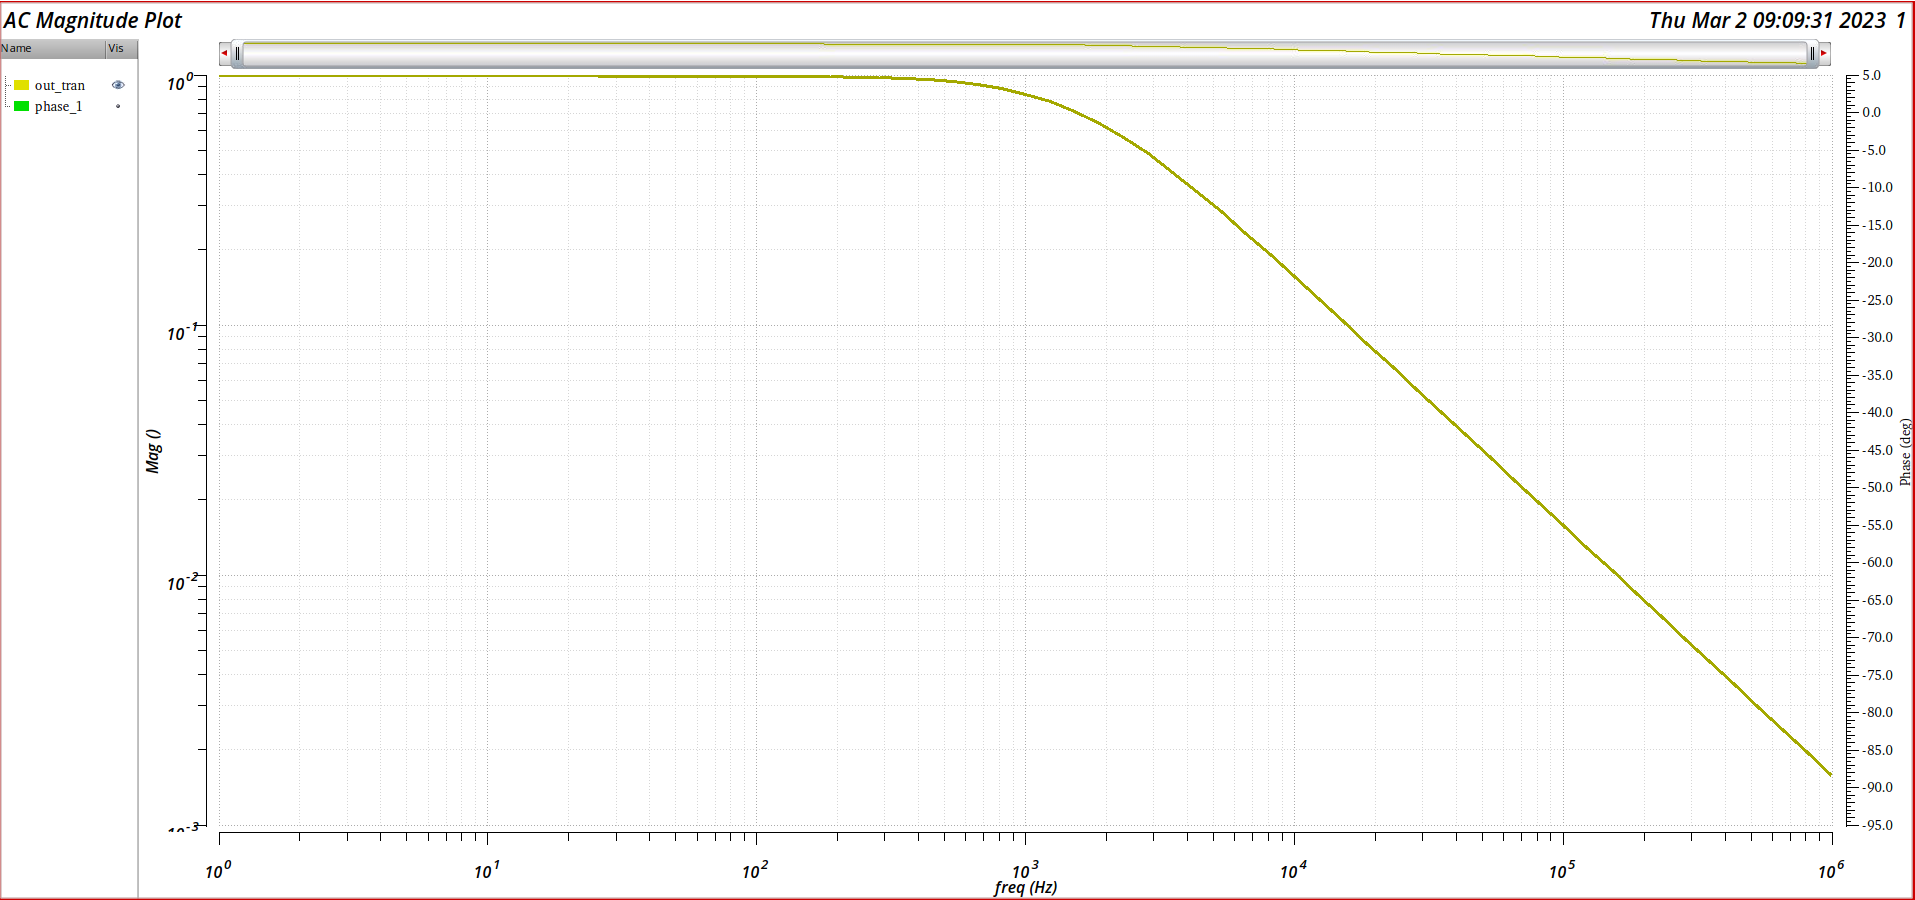
\includegraphics[width=0.7\textwidth]{./ac_sim.png}
\caption{\label{fig:ac_sim}AC magnitude plot.}
\end{figure}

\section{Parametric Analysis varying the RC Capacitance}
\label{sec:org45e9bd3}

\begin{figure}[H]
\centering
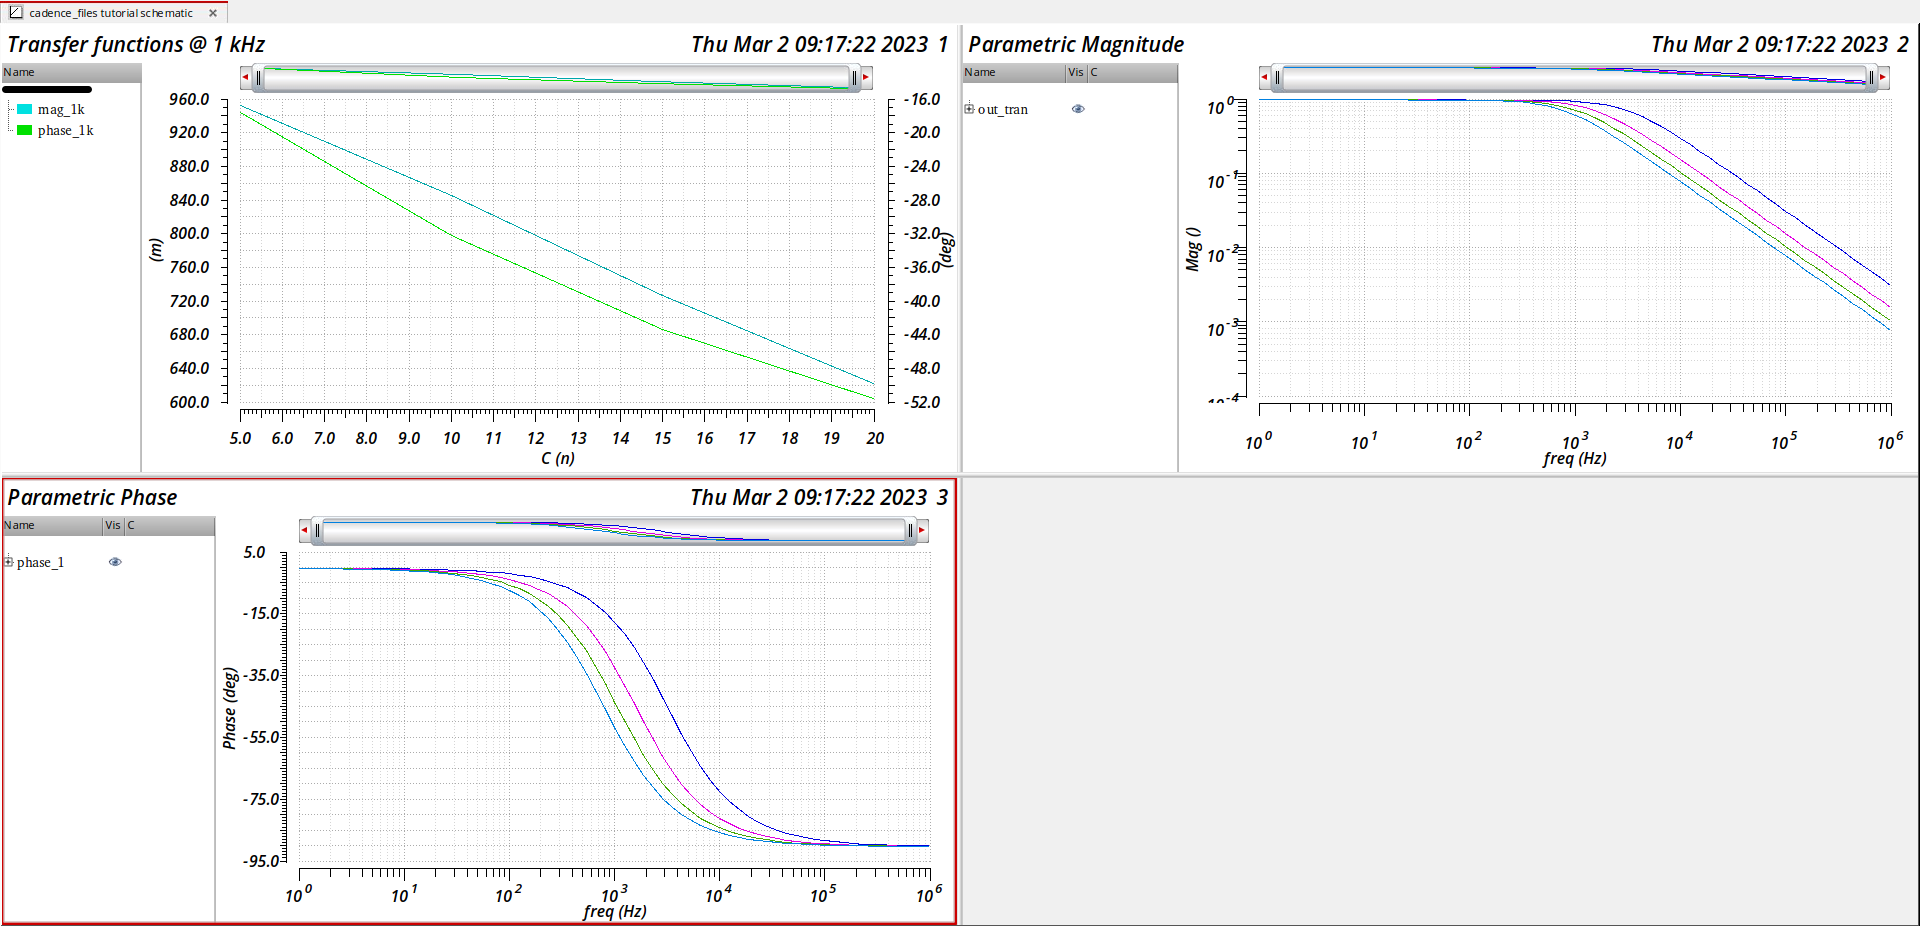
\includegraphics[width=0.7\textwidth]{./param_rc.png}
\caption{\label{fig:param_rc}All three plots.}
\end{figure}

\begin{figure}[H]
\centering
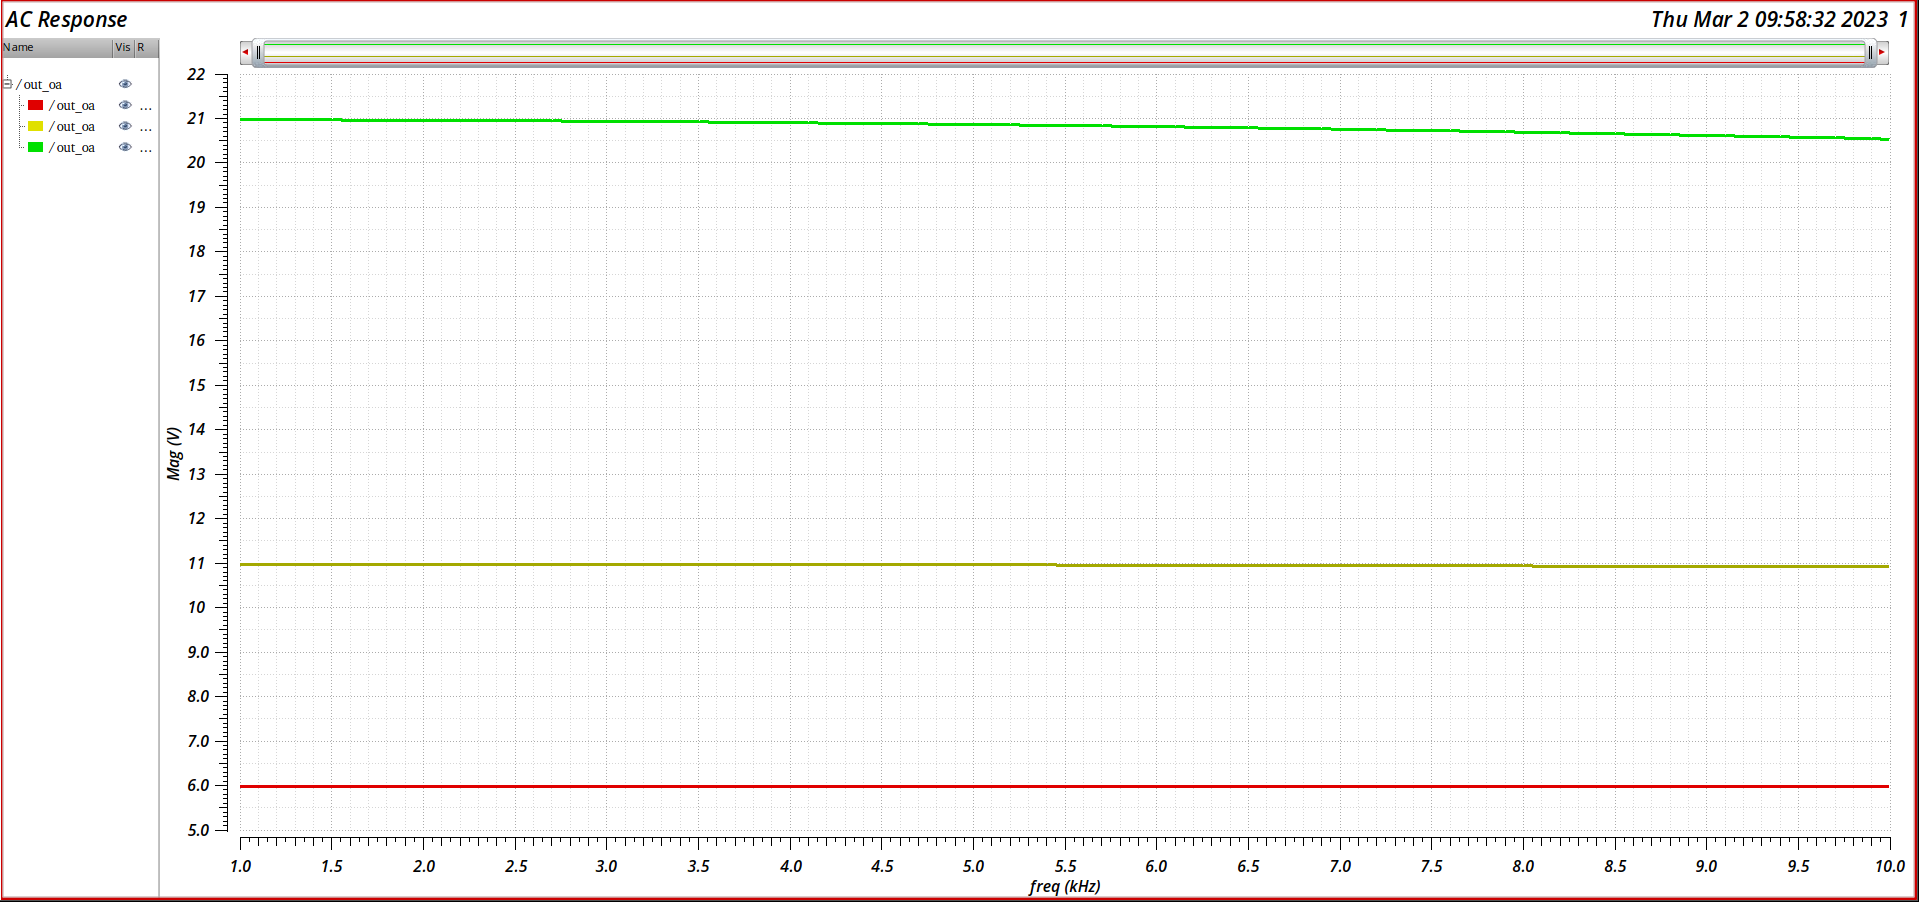
\includegraphics[width=0.7\textwidth]{./param_ac_resp.png}
\caption{\label{fig:param_ac_resp}Parametric sweep AC response.}
\end{figure}

\begin{figure}[H]
\centering
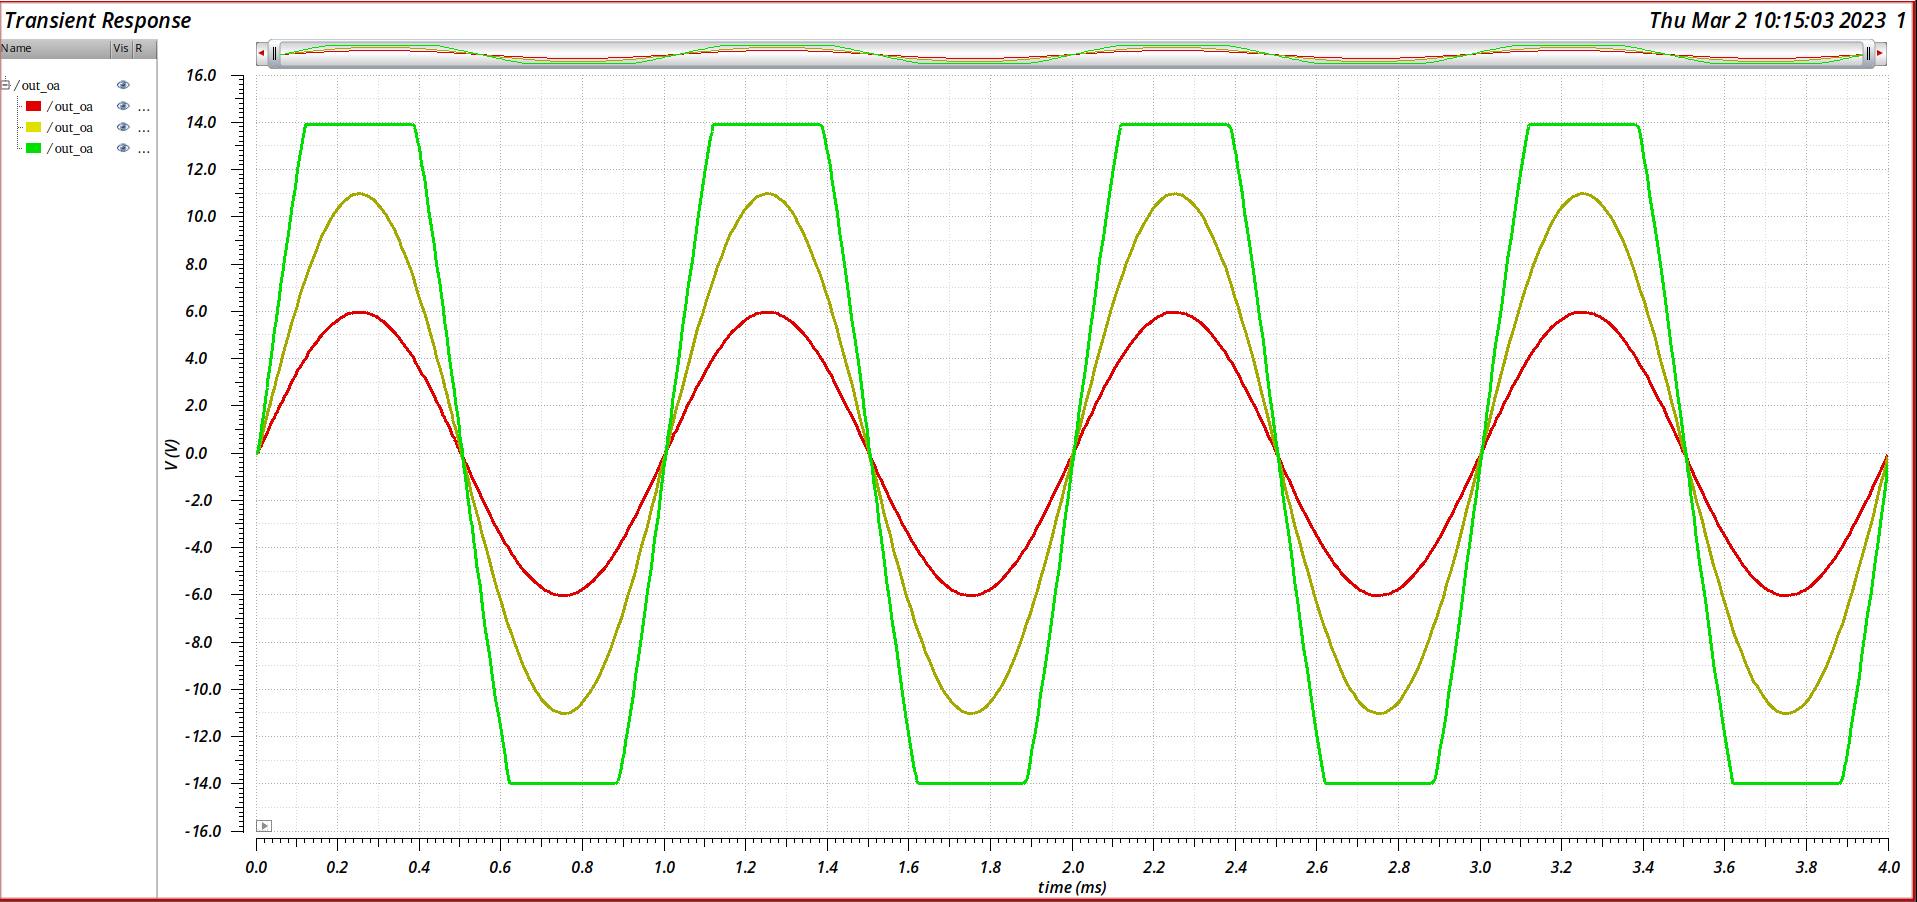
\includegraphics[width=0.7\textwidth]{./param_1k.png}
\caption{\label{fig:param_1k}Parametric sweep at \qty{1}{\kilo\hertz}.}
\end{figure}

\begin{figure}[H]
\centering
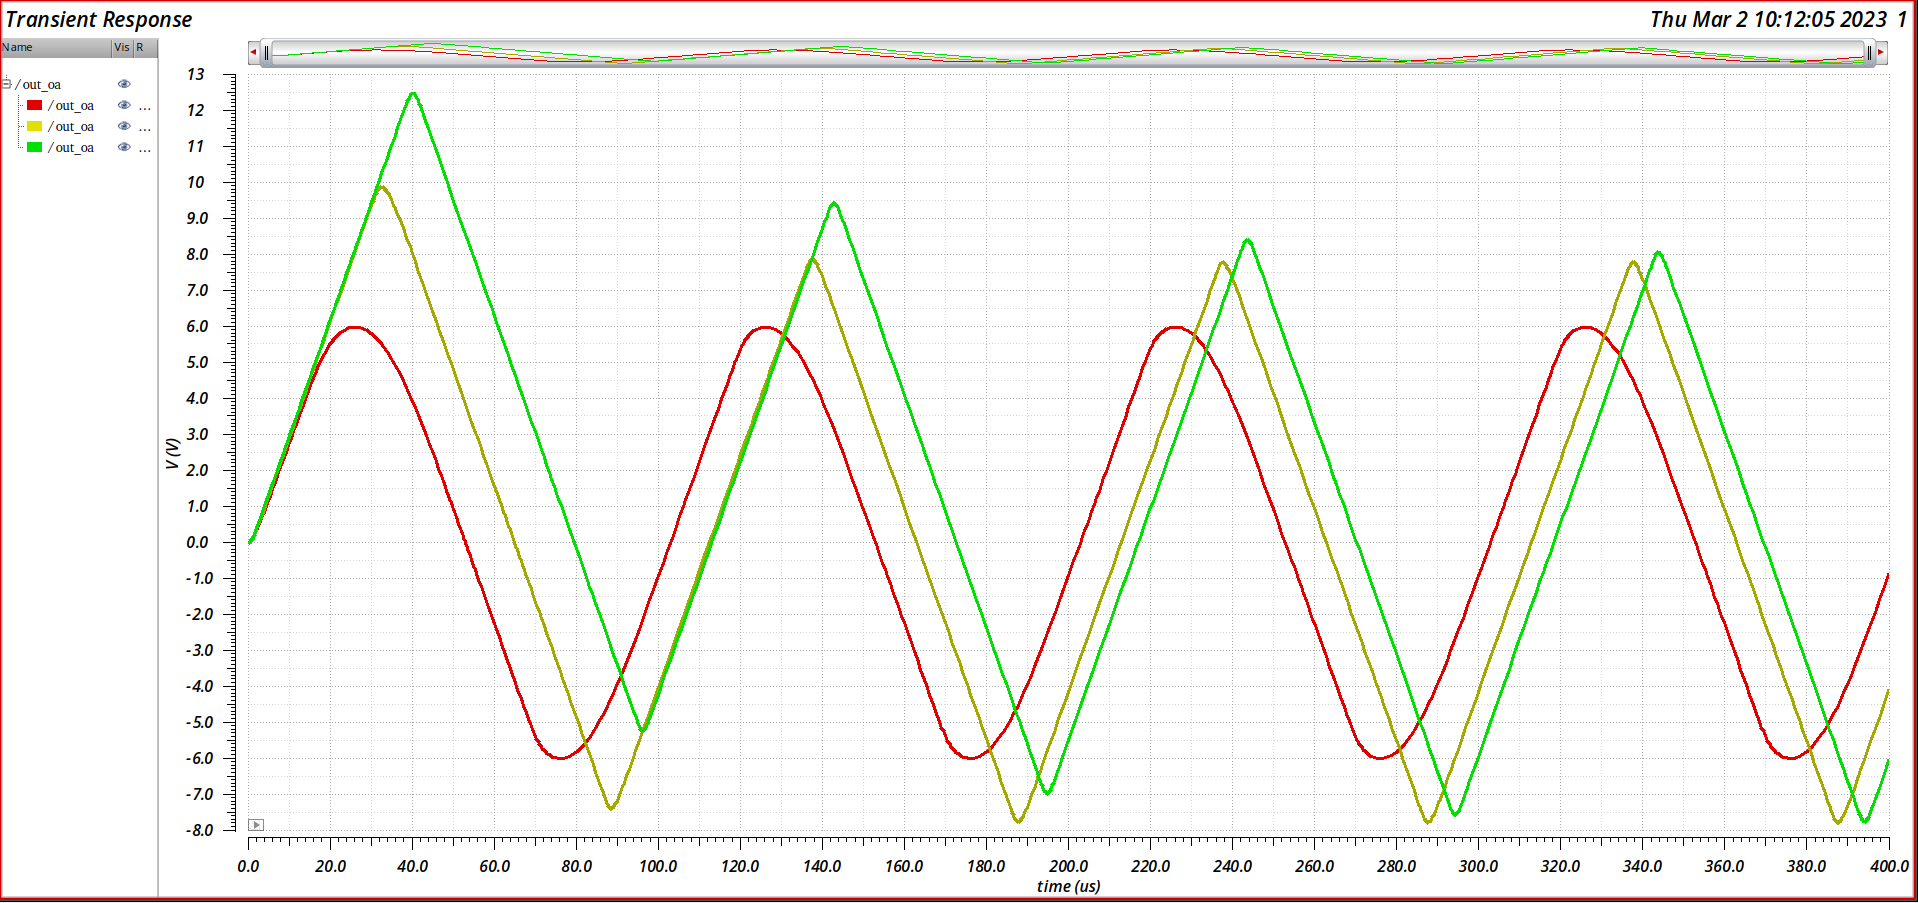
\includegraphics[width=0.7\textwidth]{./param_10k.png}
\caption{\label{fig:param_10k}Parametric sweep at \qty{10}{\kilo\hertz}.}
\end{figure}

\begin{align}
    |H(f)| &= \frac{1}{\sqrt{1 + (2\pi f RC)^2}} \\
    \angle H(f) &= \tan^{-1}(-2\pi f RC) \\
    |H(f)||_{C = \qty{10}{\nano\farad}} &= \num{0.85} \\
    |H(f)||_{C = \qty{20}{\nano\farad}} &= \num{0.62} \\
    \angle H(f)|_{C = \qty{10}{\nano\farad}} &= \ang{32.1} \\
    \angle H(f)|_{C = \qty{20}{\nano\farad}} &= \ang{51.5}
\end{align}

\section{Transient Simulation}
\label{sec:org79c1e9f}

\begin{figure}[H]
\centering
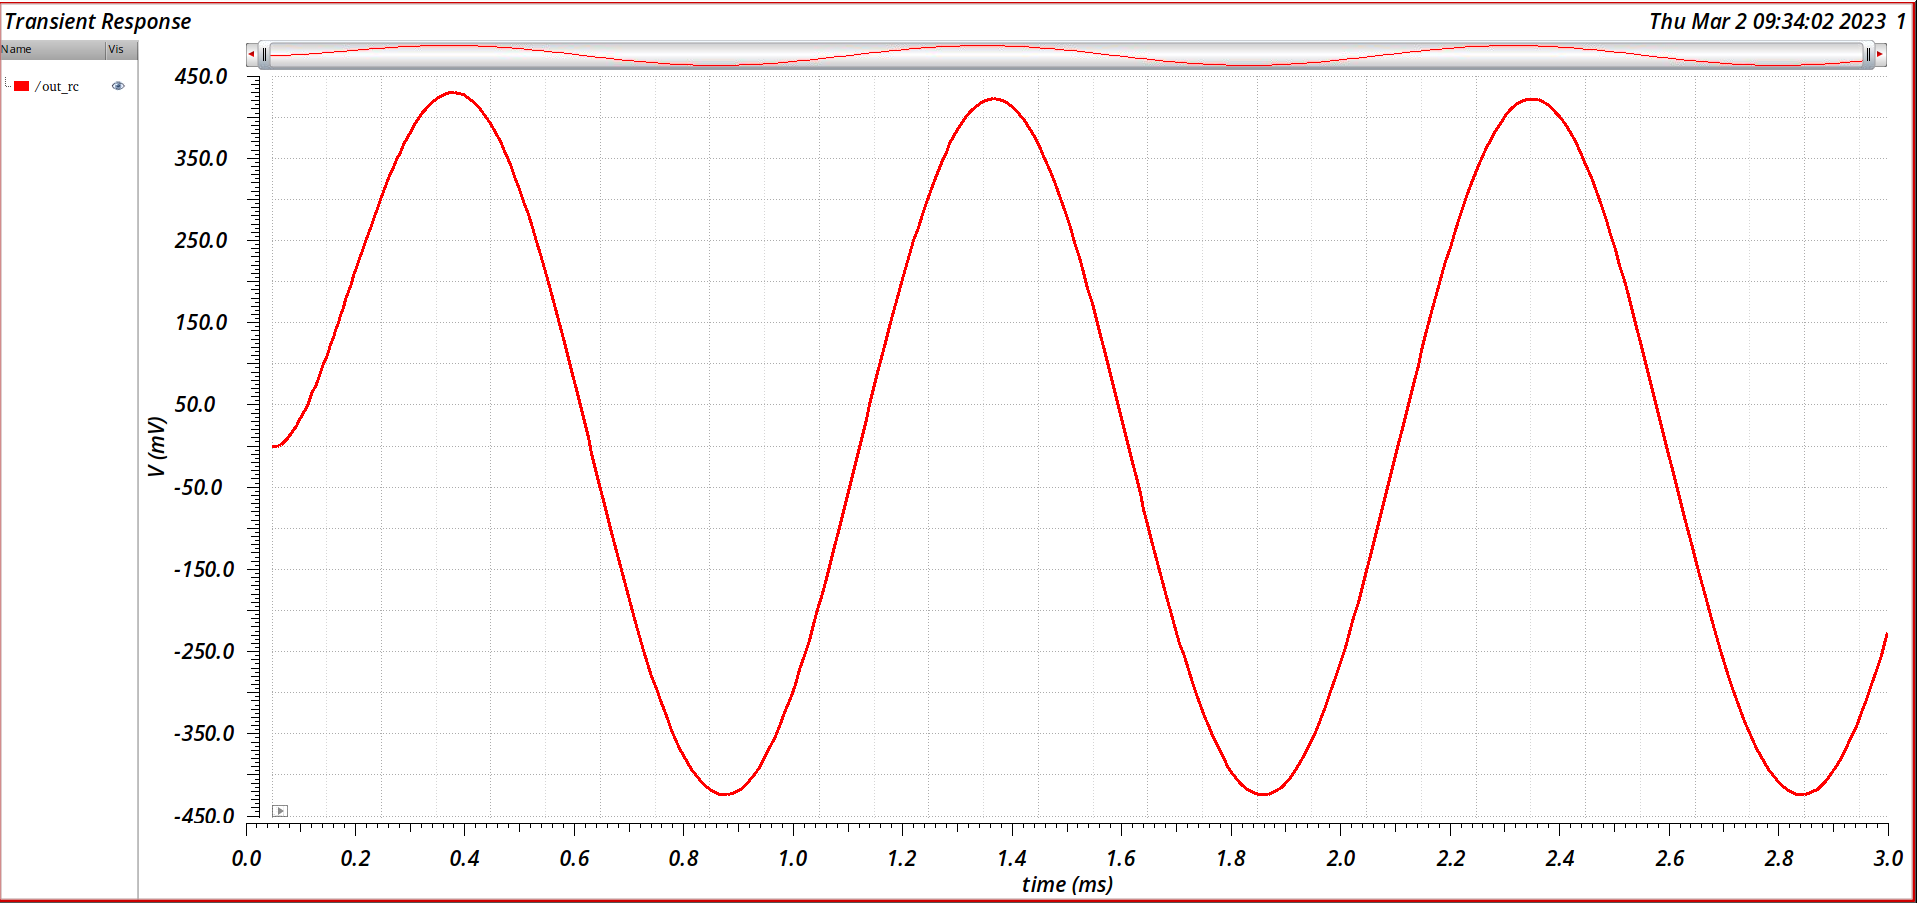
\includegraphics[width=0.7\textwidth]{./trans_rc.png}
\caption{\label{fig:trans_rc}Transient RC simulation.}
\end{figure}

\section{LM741 Simulation}
\label{sec:org7eeff03}

\begin{table}
\adjustbox{max width=\linewidth}{
\begin{center}
\begin{tabular}{llllll}
\hline
\(R\) [\unit{\kilo\ohm}] & Input Frequency [\unit{\kilo\hertz}] & Hand-Calculated Output Amplitude [\unit{\volt}] & AC Simulation Output Amplitude [\unit{\volt}] & Transient Simulation Output Amplitude [\unit{\volt}] & Circuit Output Amplitude [\unit{\volt}]\\[0pt]
\hline
\num{5} & \num{1} & \num{6} & \num{5.999} & \num{6} & \num{6.55}\\[0pt]
\num{10} & \num{1} & \num{11} & \num{10.999} & \num{11} & \num{11.55}\\[0pt]
\num{20} & \num{1} & \num{21} & \num{20.994} & \num{14} & \num{14.3}\\[0pt]
\num{5} & \num{10} & \num{6} & \num{5.990} & \num{6} & \num{6.55}\\[0pt]
\num{10} & \num{10} & \num{11} & \num{10.937} & \num{8.6} & \num{11.5}\\[0pt]
\num{20} & \num{10} & \num{21} & \num{20.560} & \num{8.8} & \num{14.3}\\[0pt]
\end{tabular}
\end{center}
}
\end{table}

\begin{table}[H]
\caption{\label{fig:5k}Output amplitudes for \(R = \qty{5}{\kilo\ohm}\). Left: \qty{1}{\kilo\hertz}. Right: \qty{10}{\kilo\hertz}.}
\centering
\begin{tabular}{ll}
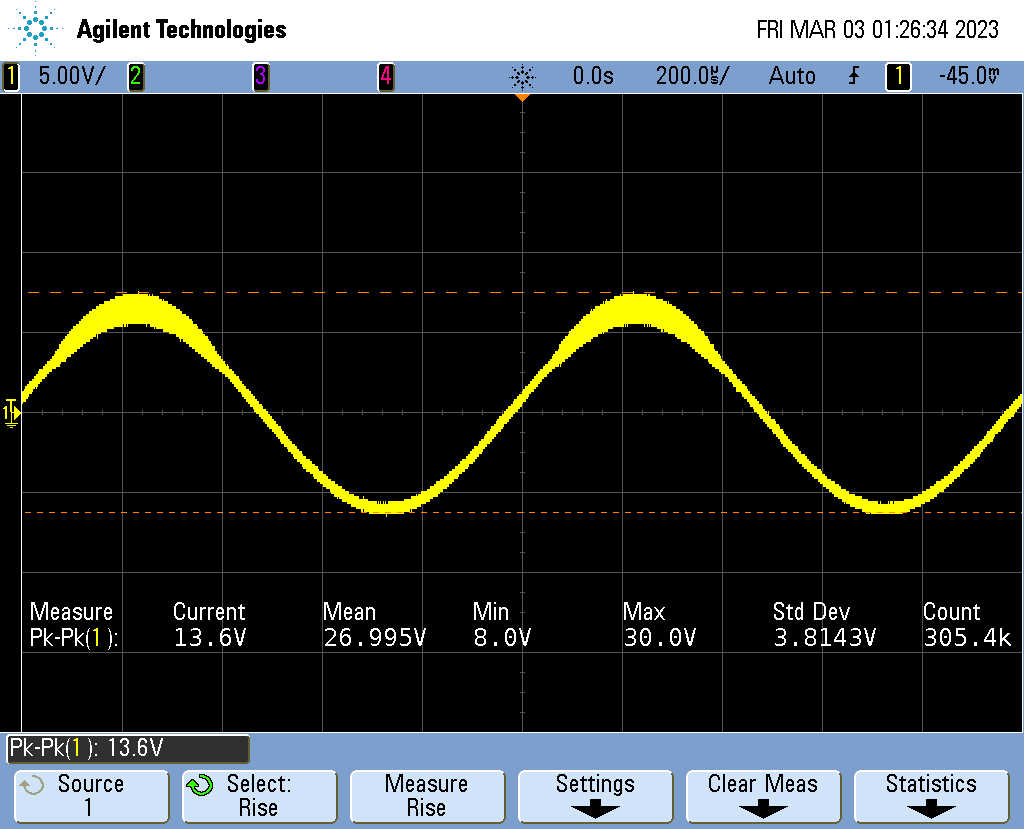
\includegraphics[width=8cm]{./5k_1k.png} & 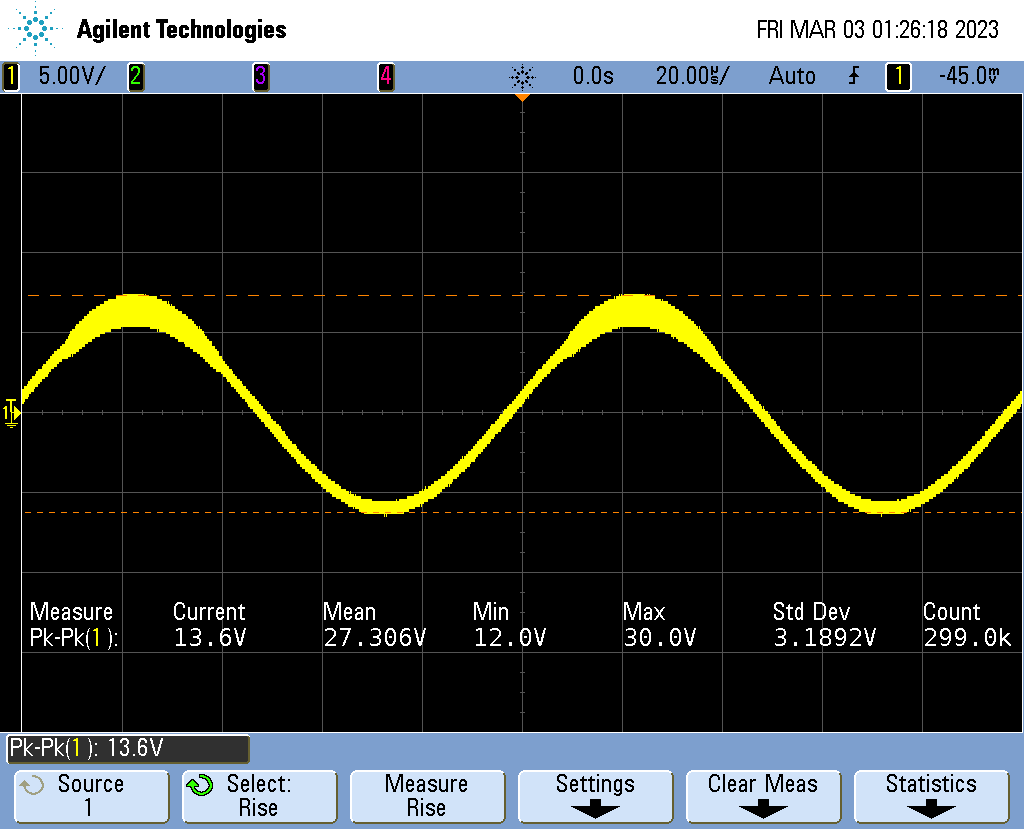
\includegraphics[width=8cm]{./5k_10k.png}\\[0pt]
\end{tabular}
\end{table}

\begin{table}[H]
\caption{\label{fig:10k}Output amplitudes for \(R = \qty{10}{\kilo\ohm}\). Left: \qty{1}{\kilo\hertz}. Right: \qty{10}{\kilo\hertz}.}
\centering
\begin{tabular}{ll}
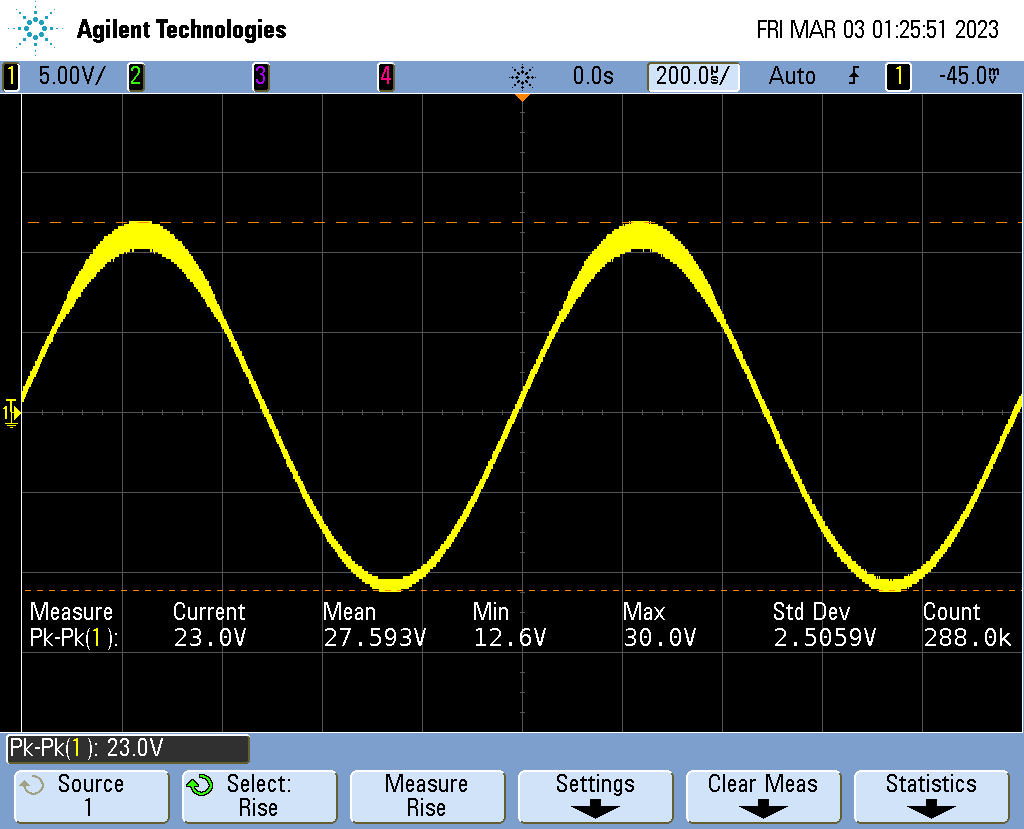
\includegraphics[width=8cm]{./10k_1k.png} & 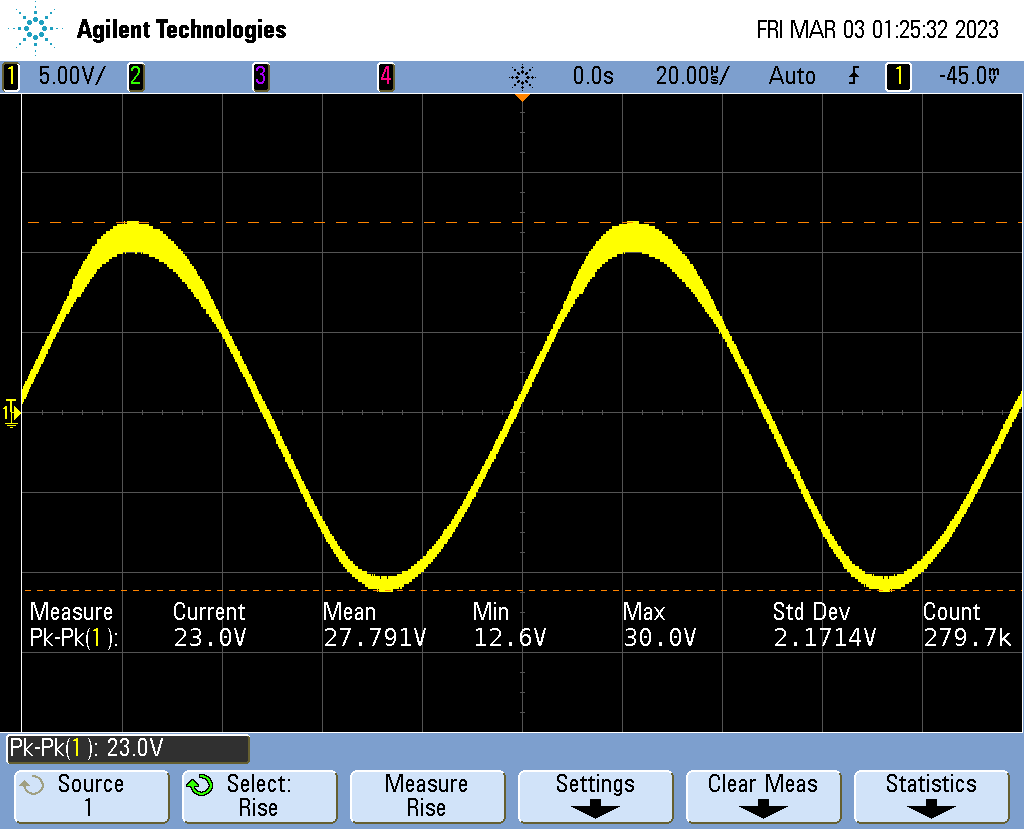
\includegraphics[width=8cm]{./10k_10k.png}\\[0pt]
\end{tabular}
\end{table}

\begin{table}[H]
\caption{\label{fig:20k}Output amplitudes for \(R = \qty{20}{\kilo\ohm}\). Left: \qty{1}{\kilo\hertz}. Right: \qty{10}{\kilo\hertz}.}
\centering
\begin{tabular}{ll}
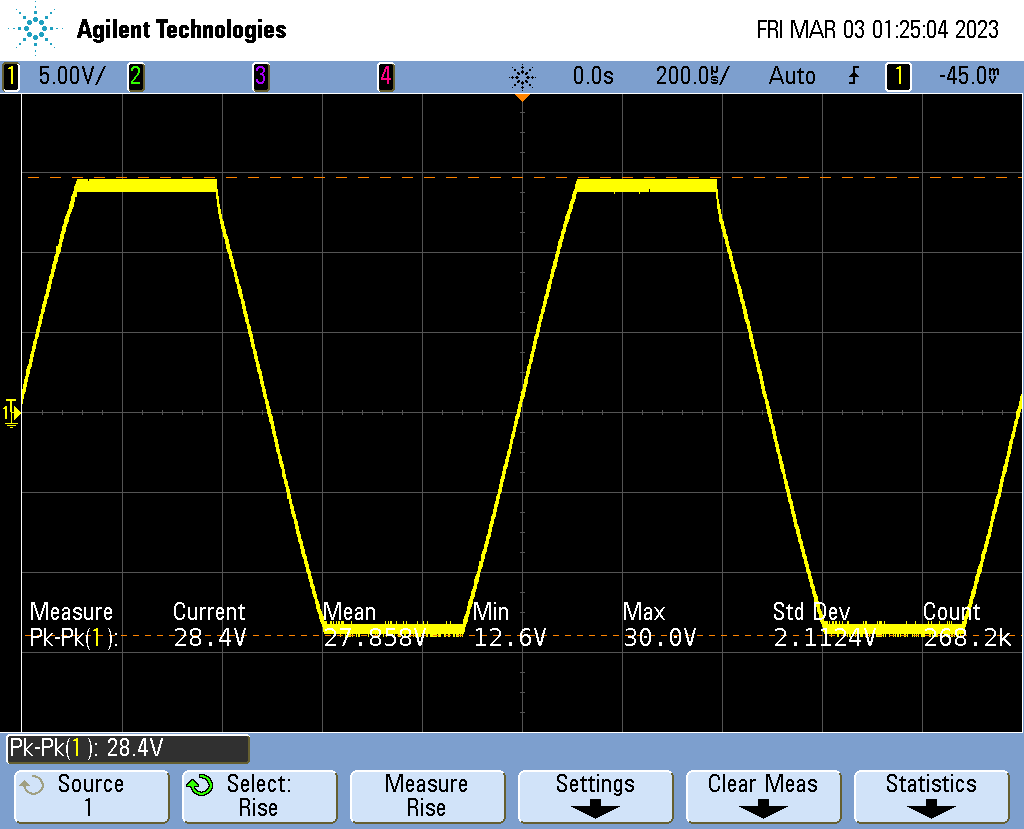
\includegraphics[width=8cm]{./20k_1k.png} & 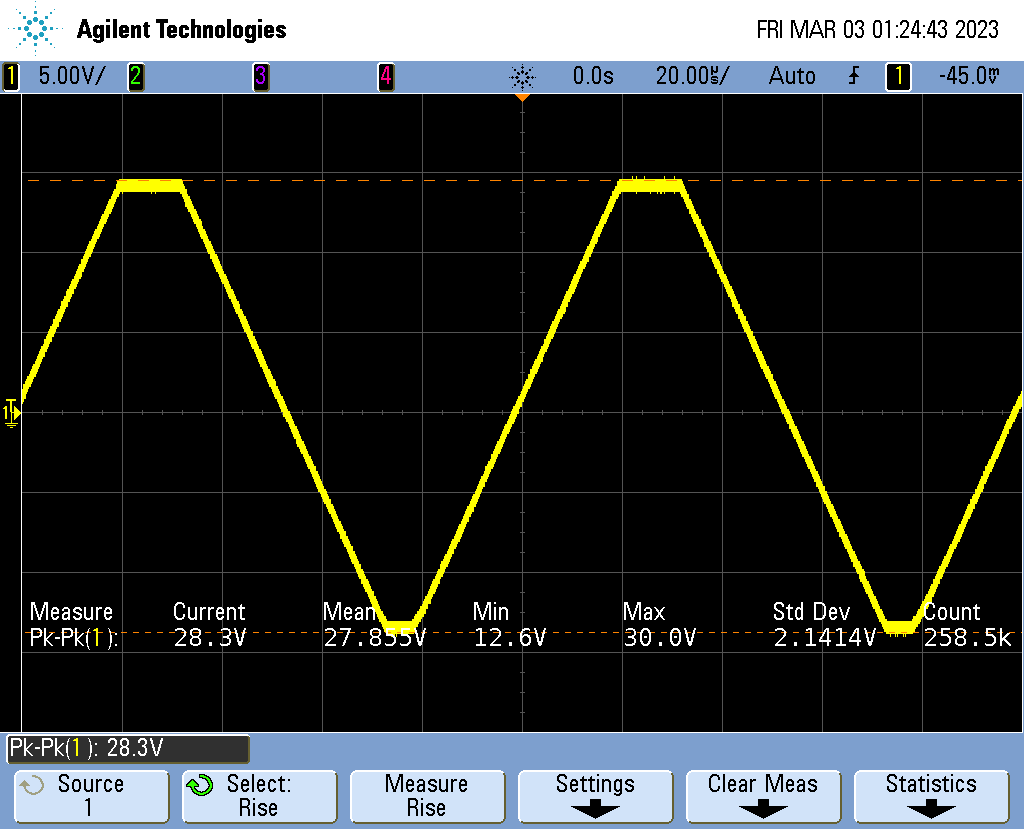
\includegraphics[width=8cm]{./20k_10k.png}\\[0pt]
\end{tabular}
\end{table}

At \qty{1}{\kilo\hertz}, the AC simulation had the greatest error.
It does not take into account the finite supply voltage.

At \qty{10}{\kilo\hertz}, the AC simulation had the greatest error.
It does not take into account the slewing of the input signal.

In hand calculation, we assume an ideal op-amp, such as infinite gain and supply voltage, as well as a non-dependence on frequency.
In AC simulation, we still maintain infinite supply voltage, but now we have a finite gain and frequency dependence.
In transient simulation, we take into account slewing as well as finite supply voltage.
This suggests that transient simulation is the closest to reality.
\end{document}